
\newpage

\section{Vectorial Semantic and Embeddings}

    Nei modelli di n-gram o di classificazione testuale, le parole erano indici o stringhe prive di contenuto semantico. Qui introduciamo l'idea che il \emph{significato} di una parola non coincide con l'etichetta simbolica, ma con il suo \emph{uso} e le relazioni che intrattiene con altre parole e con i contesti in cui appare (Wittgenstein; Harris). Questo porta ai \textbf{desiderata} per una teoria del significato: distinguere sensi, catturare relazioni (sinonimia, antonimia, similarità, relatedness), gestire connotazioni e uso nel contesto.

    \subsection{Definitions}
    
        Un \textbf{lemma} raggruppa più \textbf{wordform} flesse; ciascuna voce può essere \textbf{polisemica} (più sensi). Esempi classici mostrano lemmi con sensi tecnici e comuni (come \emph{mouse}: roditore vs. dispositivo d'ingresso). Il compito computazionale è spesso formulato come stima del senso più probabile in contesto: $\hat s = \arg\max_s P(s\mid w, C)$.\\
    
        I \textbf{sinonimi} condividono il significato in alcuni contesti (\emph{couch/sofa}, \emph{automobile/car}); ma la sinonimia perfetta è rara: differiscono per registro, polisemia, sfumature pragmatiche. Il \textbf{principio linguistico del contrasto} ricorda che differenze formali tendono a riflettere differenze di significato, scoraggiando l'idea di sinonimia assoluta.\\
        
        La \textbf{Similarità} misura quanto due parole condividano elementi di significato (\emph{cow/horse}); \textbf{relatedness} (o associazione) misura relazioni anche non somiglianti (\emph{coffee/cup}). Un criterio operativo per la similarità in modelli vettoriali è il \textbf{coseno} tra vettori semantici:
        
        $$
            \mathrm{cos}(\mathbf{v},\mathbf{w}) \,=\, \frac{\mathbf{v}\cdot\mathbf{w}}{\lVert \mathbf{v}\rVert\,\lVert \mathbf{w}\rVert} \,=\, \frac{\sum_i v_i w_i}{\sqrt{\sum_i v_i^2}\,\sqrt{\sum_i w_i^2}}.
        $$
        
        Il coseno è compreso tra $0$ e $1$ se i valori sono non negativi; normalizza per la lunghezza del vettore, correggendo il bias del prodotto scalare grezzo verso parole molto frequenti.\\

        Un \textbf{campo semantico} raccoglie parole legate da uno stesso dominio e relazioni strutturate (\emph{ristoranti: waiter, menu, chef, ...}). Il \textbf{topic modeling} (LDA) li apprende in modo non supervisionato: ogni documento è una mistura di topic, ciascun topic è una distribuzione su parole; i topic spiegano co-occorrenze senza introdurre sensi.
    
        Parole che compaiono in contesti simili tendono ad avere significati simili (Harris). La semantica vettoriale \emph{istanza} questa ipotesi costruendo rappresentazioni da co-occorrenze: matrici \textbf{term-document} o \textbf{term-term}, pesate e confrontate con misure come il coseno.\\

        L'\textbf{antonomia} è un'opposizione rispetto a una singola dimensione semantica, pur mantenendo forte affinità lessicale (\emph{hot/cold}, \emph{up/down}, \emph{rise/fall}). Gli antonimi possono definire una opposizione binaria o gli estremi di una scala gradabile; esistono anche casi \emph{reversivi} (\emph{entrare/uscire}). Nota pratica: negli spazi distribuzionali gli antonimi risultano spesso \emph{vicini} perché condividono contesti; distinguere “opposto” da “simile” richiede segnali aggiuntivi (lessici etichettati, vincoli direzionali, ecc.).\\

        \noindent Nel trattamento automatico del linguaggio naturale, i modelli statistici e neurali moderni (come i Transformer) operano su rappresentazioni numeriche delle parole, ma dietro molti sistemi di NLP classici e ibridi vi sono ancora risorse simboliche — cioè basi di conoscenza linguistiche esplicite, costruite manualmente da linguisti o semi-automaticamente.
        Tra queste, \textbf{WordNet} e \textbf{FrameNet} rappresentano due pilastri.

        \newpage
            
        \subsubsection{WordNet}

            WordNet organizza il lessico in \emph{synset}, insiemi di lemmi sinonimi che denotano un unico \emph{concetto}. Le relazioni collegano synset (non singole wordform) e includono: iponimia/iperonimia (\emph{is\!-a}), meronimia/olonimia (\emph{part\!-of}), antonimia (soprattutto per aggettivi), \emph{see\!-also}, \emph{derivationally related}, ecc. Ogni synset ha una \emph{gloss} (definizione) e talvolta esempi d'uso.

            \paragraph{Iponimia/Iperonimia (\emph{is\!-a})}
            Sia $x$ un synset “figlio” e $y$ un synset “genitore”. Scriviamo \,$x\sqsubseteq y$\, per dire che $x$ è \textbf{iponimo} di $y$ (e $y$ è \textbf{iperonimo} di $x$). La relazione \,$\sqsubseteq$\, è un ordine parziale (riflessivo, antisimmetrico, transitivo) e induce una tassonomia (albero/\,DAG) per nomi e verbi.
            
            Esempio (nomi): \;\texttt{cane} $\sqsubseteq$ \texttt{canide} $\sqsubseteq$ \texttt{carnivoro} $\sqsubseteq$ \texttt{mammifero} $\sqsubseteq$ \texttt{vertebrato}.
            
            \emph{Misure tassonomiche su WordNet}. Dati due synset $x,y$ con \emph{lowest common subsumer} (LCS) $\mathrm{lcs}(x,y)$ e profondità $\mathrm{depth}(\cdot)$ nella gerarchia, sono comuni:
            
            \begin{gather}
            \notag
            \mathrm{sim}_{\mathrm{wup}}(x,y) \,=\, \frac{2\,\mathrm{depth}(\mathrm{lcs}(x,y))}{\mathrm{depth}(x)+\mathrm{depth}(y)} \in (0,1],\\[2ex]
            \notag
            \mathrm{sim}_{\mathrm{res}}(x,y) \,=\, IC\big(\mathrm{lcs}(x,y)\big),\qquad IC(c)\,=\,-\log p(c),\\[2ex]
            \notag
            \mathrm{sim}_{\mathrm{lin}}(x,y) \,=\, \frac{2\,IC\big(\mathrm{lcs}(x,y)\big)}{IC(x)+IC(y)}
            \end{gather}
            
            Qui $p(c)$ è la probabilità empirica del concetto $c$ stimata da corpora (conteggi gerarchici). Valori più alti indicano maggiore similarità semantica.
            
            \paragraph{Meronimia/Olonimia (\emph{part\!-of})}
            La \textbf{meronimia} lega un synset parte $x$ a un synset tutto $y$ (\,$x$ \emph{part-of} \,$y$\,). In WordNet si distinguono sottotipi:
            \begin{itemize}
              \item \textit{part meronym}: parte fisica (\texttt{ruota} \,$\to$\, \texttt{auto});
              \item \textit{member meronym}: membro di un collettivo (\texttt{soldato} \,$\to$\, \texttt{esercito});
              \item \textit{substance meronym}: sostanza costituente (\texttt{cellulosa} \,$\to$\, \texttt{carta}).
            \end{itemize}
            L'olonimia è l'inversa (\emph{has\!-part}). A differenza dell'iponimia, \emph{part\!-of} non definisce una tassonomia ma una gerarchia \emph{partitiva}. È utile per inferenze “parte\,\,$\leftrightarrow$\,tutto” e per task di IE (estrazione relazioni).
            
            \paragraph{Altre relazioni essenziali}
            \begin{center}
                \begin{tabular}{@{}lll@{}}
                    \toprule
                    \textbf{Relazione} & \textbf{Tipo} & \textbf{Esempio} \\
                    \midrule
                    Antonymy & opposizione & \texttt{caldo} vs. \texttt{freddo} (aggettivi) \\
                    Derivationally related & morfologica & \texttt{govern} $\leftrightarrow$ \texttt{government} \\
                    Also-see & semantica debole & \texttt{chirurgo} \,$\to$\, \texttt{medico} \\
                    Verb entailment & implicazione & \texttt{snore} \,$\Rightarrow$\, \texttt{sleep} \\
                    \bottomrule
                \end{tabular}
            \end{center}
            
            \paragraph{Lesk (gloss overlap)}
            Per sfruttare le \emph{gloss}, il criterio di Lesk disambigua scegliendo il senso con massima sovrapposizione tra parole della definizione e del contesto. Sia $G(s)$ l'insieme (o multinsieme) di lemmi nella gloss del senso $s$ e $C$ i lemmi di contesto: si seleziona $\hat s=\arg\max_s |G(s)\cap C|$ (o versioni pesate), utile come baseline per WSD.

        \newpage
            
        \subsubsection{FrameNet}
        
            FrameNet cattura \textbf{frame} concettuali (schemi di situazioni) con i loro ruoli \textbf{Frame Elements (FE)} e le \textbf{Lexical Units (LU)} che li evocano. Un frame modella una scena prototipica (\emph{Commercio}, \emph{Viaggio}, \emph{Causa\_morte}, ...).
            
            \paragraph{Componenti principali}
            
            \begin{itemize}
            
              \item \textbf{Frame}. Struttura concettuale: es. \emph{Commercial\_transaction}.
              
              \item \textbf{Frame Elements}. Ruoli semantici (core/non\!-core): es. \emph{Buyer}, \emph{Seller}, \emph{Goods}, \emph{Money}, \emph{Time}.
              
              \item \textbf{Lexical Units}. Coppie (lemma, POS) che evocano il frame: es. \texttt{buy.v}, \texttt{purchase.v}, \texttt{sell.v} (quest'ultima può evocare un frame prospettico diverso, es. \emph{Commerce\_sell}).
              
            \end{itemize}
            
            L'annotazione FrameNet indica per ogni frase quali FE sono realizzati e con quali span.
            
            \paragraph{Relazioni tra frame}
            
            \begin{center}
                \begin{tabular}{@{}lll@{}}
                    \toprule
                    \textbf{Relazione} & \textbf{Intuizione} & \textbf{Esempio} \\
                    \midrule
                    Inheritance & specializzazione di un frame & \emph{Hiring} \,$\sqsubseteq$\, \emph{Commercial\_transaction} \\
                    Using & un frame usa lo schema di un altro & \emph{Buying} \emph{uses} \emph{Possession} \\
                    Perspective\_on & prospettive complementari & \emph{Commerce\_sell} vs. \emph{Commerce\_buy} \\
                    Subframe & sotto\!-evento incluso & \emph{Travel} include \emph{Departing}, \emph{Arriving} \\
                    Precedes/Causative\_of & ordine causale/temporale & \emph{Paying} precede \emph{Owning} \\
                    \bottomrule
                \end{tabular}
            \end{center}
            
        \subsection*{WordNet vs FrameNet}
        
            WordNet fornisce un \emph{inventario di concetti e relazioni lessicali} (sinonimia, tassonomie e partonomie) utile per misurare similarità e per WSD. FrameNet modella \emph{scene e ruoli} utili per SRL (Semantic Role Labeling), IE e comprensione a livello di evento. Le due risorse sono complementari: synset per “cosa è” \,(\emph{is\!-a}) e frame per “cosa accade e chi partecipa”.

        \newpage
        
        \subsubsection{Sentiment Connotation}
            
            Per una parola $w$ definiamo una rappresentazione connotativa di base come
            
            $$
                \mathrm{con}(w) \,=\, \big(\mathrm{pol}(w),\, \mathrm{int}(w)\big),\qquad \mathrm{pol}(w)\in[-1,1],\ \mathrm{int}(w)\in[0,1]
            $$
            
            \textbf{Polarità} ($-1$ negativa, $+1$ positiva) e \textbf{intensità} (forza del segno).\\
            
            \begin{wrapfigure}{r}{0.5\textwidth}
                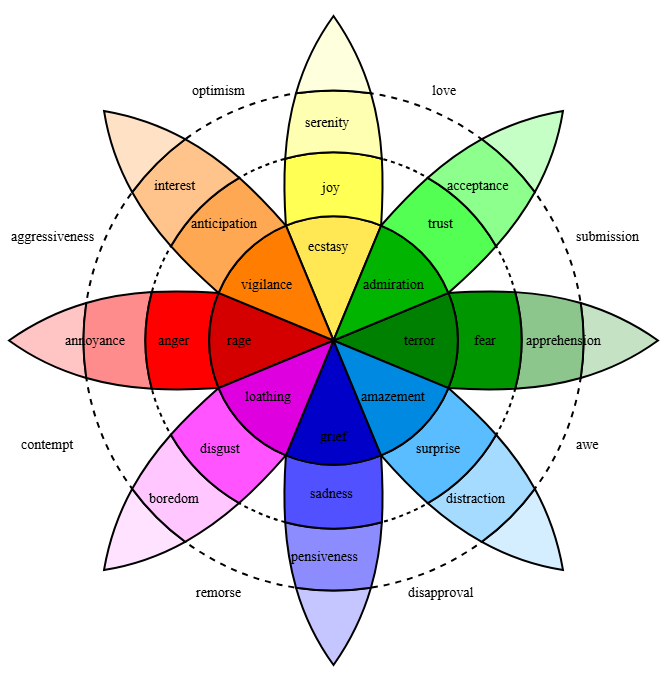
\includegraphics[width=1\linewidth]{imgs/schema_5_1.png}
                \label{fig:fig51}
                \caption{Plutchick's wheel of emotion}
            \end{wrapfigure}
            
            Se disponibile, si può estendere a coordinate affettive \textbf{VAD} (\emph{Valence–Arousal–Dominance}); esse rappresentano la connotazione emotiva su tre assi continui: \emph{Valence} misura il grado edonico (spiacevole $\to$ piacevole), \emph{Arousal} l'attivazione (calmo $\to$ eccitato), \emph{Dominance} il senso di controllo/potere (sottomesso $\to$ dominante). Per una parola $w$ definiamo un vettore $\,\mathbf{v}(w)\in\mathbb{R}^3\,$ (normalizzato in $[0,1]$ o centrato in $[-1,1]$). Lo score di una frase/documento $d=w_{1:N}$ si ottiene per media, eventualmente pesata, delle coordinate:
            
            $$
            \mathbf{v}(d)=\frac{1}{Z}\sum_{i=1}^{N}\alpha_i\,\mathbf{v}(w_i),\qquad \alpha_i\ge 0,\ \ Z=\sum_i \alpha_i,
            $$
            
            dove i pesi $\alpha_i$ possono riflettere POS, distanza dal target o salienza sintattica. La composizione locale gestisce negazioni e intensificatori scalando le componenti (es.: $\mathrm{neg}(x):\, v_{\text{V}}\!\leftarrow\!-\lambda\,v_{\text{V}}$; $\mathrm{molto}(x):\, \mathbf{v}\!\leftarrow\!\kappa\,\mathbf{v}$ con $0<\lambda\le1,\ \kappa>1$).\\
            
            \noindent Dato un testo $d=w_{1:N}$ e un lessico connotativo (prior di parola), uno score medio è

            $$
                s(d) \,=\, \frac{1}{N}\sum_{i=1}^{N} \mathrm{pol}(w_i),\qquad s(d)\in[-1,1]
            $$
            
            Per dare più peso ai token informativi, si introducono pesi $\alpha_i\ge 0$ con $\sum_i \alpha_i=1$ (in base a POS, dipendenze, distanza dal target):

            $$
                s_{\alpha}(d) \,=\, \sum_{i=1}^{N} \alpha_i\,\mathrm{pol}(w_i).
            $$
            
            Le connotazioni si \emph{compongono} nel contesto. Su una finestra di scope (meglio: arco di dipendenza) definiamo trasformazioni semplici:
            
            \begin{align}
                 \notag\mathrm{pol}(\text{neg }x) &\;=\; -\lambda\,\mathrm{pol}(x), && 0<\lambda\le 1,\\
                 \notag\mathrm{pol}(\text{molto }x) &\;=\; \kappa\,\mathrm{pol}(x), && \kappa>1,\\
                 \notag\mathrm{pol}(\text{poco }x) &\;=\; \mu\,\mathrm{pol}(x), && 0<\mu<1.
            \end{align}
            
            Esempi: \emph{non buono} $\Rightarrow$ attenuazione/inversione ($\lambda\lesssim 1$); \emph{molto utile} $\Rightarrow$ amplificazione ($\kappa>1$); \emph{poco convincente} $\Rightarrow$ attenuazione ($\mu<1$). Nella pratica si usa un insieme di segnali (lista di negazioni, intensificatori, attenuatori) e si limita lo \emph{scope} con regole sintattiche per evitare inversioni spurie.
    
    \newpage

    \subsection{Vector Semantics}
    
        La \emph{vector semantics} rappresenta il significato delle parole tramite vettori numerici in uno spazio $\mathbb{R}^d$. A ciascuna parola $w$ associamo un vettore denso $\mathbf{e}(w)\in\mathbb{R}^d$ tale che parole con significati simili risultino vicine secondo una misura di similarità (di solito la coseno):
        
        $$
        \mathrm{sim}(w_i,w_j) \,=\, \cos\!\big(\mathbf{e}(w_i),\mathbf{e}(w_j)\big) \,=\, \frac{\mathbf{e}(w_i)\cdot\mathbf{e}(w_j)}{\lVert\mathbf{e}(w_i)\rVert\,\lVert\mathbf{e}(w_j)\rVert}
        $$
        
        L'idea chiave è distribuzionale: parole che compaiono in contesti simili hanno rappresentazioni simili.\\
        
        \noindent Esistono due vie principali, concettualmente semplici, per ottenere vettori semantici:

        \begin{itemize}
        
            \item\textbf{Conteggi e matrici (count–based).} Si costruisce una matrice parola–contesto $\mathbf{M}\in\mathbb{R}^{|V|\times|\mathcal{C}|}$ a partire dalle co–occorrenze $\mathrm{count}(w,c)$ in finestre o dipendenze; si trasformano le celle con un peso informativo (es. PMI/PPMI) e, opzionalmente, si riduce la dimensionalità con SVD per ottenere vettori densi:
            
            $$
            \mathrm{PMI}(w,c)=\log\frac{P(w,c)}{P(w)P(c)},\qquad \mathrm{PPMI}(w,c)=\max\big(\mathrm{PMI}(w,c),0\big),
            $$
            
            $$ \mathbf{M}\approx\mathbf{U}_k\,\mathbf{\Sigma}_k\,\mathbf{V}_k^{\top},\quad \text{vettore parola } \mathbf{e}(w)=\big(\mathbf{U}_k\mathbf{\Sigma}_k^{p}\big)_{w,:},\ p\in\{0,\tfrac12,1\}
            $$
        
            Questa famiglia è trasparente: i vettori derivano direttamente dalle statistiche di co–occorrenza.
        
            \item\textbf{Predittivi (neural/predictive).} Invece di contare, si \emph{apprendono} i vettori come parametri che rendono buone le previsioni di contesto o della parola. In forma astratta, dato un obiettivo predittivo $\mathcal{J}(\theta)$ su coppie (parola, contesto), si ottimizzano parametri $\theta$ (tra cui i vettori) per massimizzare la verosimiglianza o una loss contrastiva; il risultato sono embedding $\mathbf{e}(w)$ che catturano regolarità distribuzionali. Esempi classici sono modelli che predicono $P(w\mid C)$ o $P(C\mid w)$ con una testa softmax e normalizzazione:
            
            $$
            P(w\mid C)\;=\;\frac{\exp\big(\mathbf{e}(w)\cdot\mathbf{g}(C)\big)}{\sum_{w'\in V}\exp\big(\mathbf{e}(w')\cdot\mathbf{g}(C)\big)}
            $$
        
            con $\mathbf{g}(C)$ vettore del contesto. Gli embedding sono le righe (o colonne) delle matrici dei parametri.
        
        \end{itemize}
        
        Un \textbf{embedding} è una mappa $\mathrm{emb}: V \to \mathbb{R}^d$ che associa a ogni parola $w\in V$ un vettore $\mathbf{e}(w)$. Questi vettori sono \emph{densi}, a bassa dimensione ($d\ll |V|$), e permettono di eseguire calcoli geometrici (similarità, distanza, analogie) e di fungere da input numerico per modelli supervisionati/neurali. Il principio operativo è che proprietà semantiche e sintagmatiche della parola emergono come \emph{direzioni} e \emph{vicinanze} nello spazio: parole con ruoli simili hanno vettori vicini, trasformazioni lineari catturano relazioni regolari, e la composizione (es. medie pesate) consente di costruire rappresentazioni per frasi brevi.\\
